\documentclass{beamer}

\usepackage{beamerthemesplit}
\usepackage{graphicx}
\usepackage{color, natbib, hyperref}
\usepackage{bibentry}
\nobibliography*

% Algorithm environment
\usepackage{algpseudocode,algorithm,algorithmicx}
\newcommand*\Let[2]{\State #1 $\gets$ #2}


% define colors
\definecolor{jblue}  {RGB}{20,50,100}
\definecolor{ngreen} {RGB}{98,158,31}

%theme

\usetheme{boxes} 
%\usecolortheme{seahorse} 
\setbeamertemplate{items}[default] 
%\setbeamercovered{transparent}
\setbeamertemplate{blocks}[rounded]
\setbeamertemplate{navigation symbols}{} 
% set the basic colors
\setbeamercolor{palette primary}   {fg=black,bg=white}
\setbeamercolor{palette secondary} {fg=black,bg=white}
\setbeamercolor{palette tertiary}  {bg=jblue,fg=white}
\setbeamercolor{palette quaternary}{fg=black,bg=white}
\setbeamercolor{structure}{fg=jblue}
\setbeamercolor{titlelike}         {bg=jblue,fg=white}
\setbeamercolor{frametitle}        {bg=jblue!10,fg=jblue}
\setbeamercolor{cboxb}{fg=black,bg=jblue}
\setbeamercolor{cboxr}{fg=black,bg=red}

% reduce space before/after equations
\expandafter\def\expandafter\normalsize\expandafter{%
    \normalsize
    \setlength\abovedisplayskip{1pt}
    \setlength\belowdisplayskip{1pt}
    \setlength\abovedisplayshortskip{1pt}
    \setlength\belowdisplayshortskip{1pt}
}

% set colors for itemize/enumerate
\setbeamercolor{item}{fg=ngreen}
\setbeamercolor{item projected}{fg=white,bg=ngreen}

% set colors for blocks
\setbeamercolor{block title}{fg=ngreen,bg=white}
\setbeamercolor{block body}{fg=black,bg=jblue!10}

% set colors for alerted blocks (blocks with frame)
\setbeamercolor{block alerted title}{fg=white,bg=jblue}
\setbeamercolor{block alerted body}{fg=black,bg=jblue!10}
\setbeamercolor{block alerted title}{fg=white,bg=dblue!70} % Colors of the highlighted block titles
\setbeamercolor{block alerted body}{fg=black,bg=dblue!10} % Colors of the body of highlighted blocks

% set the fonts
\usefonttheme{professionalfonts}

\setbeamerfont{section in head/foot}{series=\bfseries}
\setbeamerfont{block title}{series=\bfseries}
\setbeamerfont{block alerted title}{series=\bfseries}
\setbeamerfont{frametitle}{series=\bfseries}
\setbeamerfont{frametitle}{size=\Large}
\setbeamerfont{block body}{series=\mdseries}
\setbeamerfont{caption}{series=\mdseries}
\setbeamerfont{headline}{series=\mdseries}


% set some beamer theme options
\setbeamertemplate{title page}[default][colsep=-4bp,rounded=true]
\setbeamertemplate{sections/subsections in toc}[square]
\setbeamertemplate{items}[circle]
\setbeamertemplate{blocks}[width=0.0]
\beamertemplatenavigationsymbolsempty

% Making a DAG
\usepackage{tkz-graph}  
\usetikzlibrary{shapes.geometric}
\usetikzlibrary{positioning}
\tikzstyle{VertexStyle} = [shape            = rectangle,
                               minimum width    = 6ex,%
                               draw]
 \tikzstyle{EdgeStyle}   = [->,>=stealth']      

% Define block styles
\tikzstyle{f} = [rectangle, draw, fill=blue!20, 
    text width=3em, text badly centered, node distance=1.75cm]
\tikzstyle{message} = [rectangle, draw, fill=green!20, 
    text width=3em, text centered]
\tikzstyle{io} = [draw, circle,fill=red!20, node distance=2cm,
    minimum height=2em]
\tikzstyle{line} = [draw, -latex']

% Math macros
\newcommand{\cD}{{\mathcal D}}
\newcommand{\cF}{{\mathcal F}}
\newcommand{\todo}[1]{{\color{red}{TO DO: \sc #1}}}

\newcommand{\reals}{\mathbb{R}}
\newcommand{\integers}{\mathbb{Z}}
\newcommand{\naturals}{\mathbb{N}}
\newcommand{\rationals}{\mathbb{Q}}

\newcommand{\ind}[1]{1_{#1}} % Indicator function
\newcommand{\pr}{\mathbb{P}} % Generic probability
\newcommand{\ex}{\mathbb{E}} % Generic expectation
\newcommand{\var}{\textrm{Var}}
\newcommand{\cov}{\textrm{Cov}}

\newcommand{\normal}{N} % for normal distribution (can probably skip this)
\newcommand{\eps}{\varepsilon}
\newcommand\independent{\protect\mathpalette{\protect\independenT}{\perp}}
\def\independenT#1#2{\mathrel{\rlap{$#1#2$}\mkern2mu{#1#2}}}

\newcommand{\convd}{\stackrel{d}{\longrightarrow}} % convergence in distribution/law/measure
\newcommand{\convp}{\stackrel{P}{\longrightarrow}} % convergence in probability
\newcommand{\convas}{\stackrel{\textrm{a.s.}}{\longrightarrow}} % convergence almost surely

\newcommand{\eqd}{\stackrel{d}{=}} % equal in distribution/law/measure
\newcommand{\argmax}{\arg\!\max}
\newcommand{\argmin}{\arg\!\min}

\newcommand{\bit}{\begin{itemize}}
\newcommand{\eit}{\end{itemize}}


\mode<presentation>

\title[Simple Random Sampling: Not So Simple]{Simple Random Sampling: Not So Simple}
\author{Kellie Ottoboni \\ with Philip B.~Stark and Ron Rivest}
\institute[]{Department of Statistics, UC Berkeley\\Berkeley Institute for Data Science}
\date{Qualifying Exam \\ January 23, 2017}

\begin{document}

\frame{
\titlepage
\vfill
\begin{columns}[T]
\begin{column}{.5\textwidth}
\begin{center}
\vspace{25pt}

\includegraphics[width=\textwidth]{fig/logo/dept1.pdf}
\end{center}
\end{column}
\begin{column}{.3\textwidth}
\begin{center}
\end{center}
\end{column}
\begin{column}{.3\textwidth}
\begin{center}

\includegraphics[width=0.9\textwidth]{fig/logo/BIDS.png}
\end{center}
\end{column}
\end{columns}
}



\section[Introduction]{Introduction}

\frame{
\frametitle{Simple Random Sampling}
\bit
\item Sampling is at the heart of Statistics
\bit
\item Frequentist methods: uncertainty is quantified over theoretical repeated samples
\item Surveys, audits: population is too large, so a representative sample is used instead
\eit
\item \textbf{Simple random sampling:} drawing $k$ objects from a group of $n$ in such a way that all $n\choose k$ possible subsets are equally likely
\eit
}

\frame{
\frametitle{Simple Random Sampling}
In practice, it is difficult to draw truly random samples.
\vspace{20pt}

Instead, people tend to draw samples using
\bit
\item A \textbf{pseudo-random number generator} (PRNG) 
\item An algorithm that maps a set of pseudo-random numbers into a subset of the population
\eit
\vspace{20pt}

Statisticians take for granted that this procedure is a sufficient approximation to simple random sampling.
}


%\frame
%{
%  \frametitle{PRNGs}
%  
%  \textbf{Pseudorandom number generator:} a deterministic algorithm that produces sequences that are computationally indistinguishable from the uniform distribution
%%\begin{center}
%%\begin{itemize}
%%\item \textbf{Simple random sampling:} drawing $k \le n$ items from a population of $n$ items, in such a way that each of the $n \choose k$ subsets of size $k$ is equally likely.
%%\item Difficult to obtain truly random samples. Instead, use \textbf{pseudorandom number generators (PRNGs)} to select items
%%\item \textbf{Pseudorandom}: computationally indistinguishable from the uniform distribution
%%\end{itemize}
%%\end{center}
%%
%%Good PRNGs produce pseudorandom sequences. Do they give simple random samples with equal probabilities?
%
%}

\frame{
\frametitle{Pigeons and Pigeonholes}

\begin{theorem}[Pigeonhole Principle]
If there are $n$ pigeonholes and $m>n$ pigeons, then there exists at least one pigeonhole containing more than one pigeon.
\end{theorem}
\begin{figure}[htbp]
\begin{center}
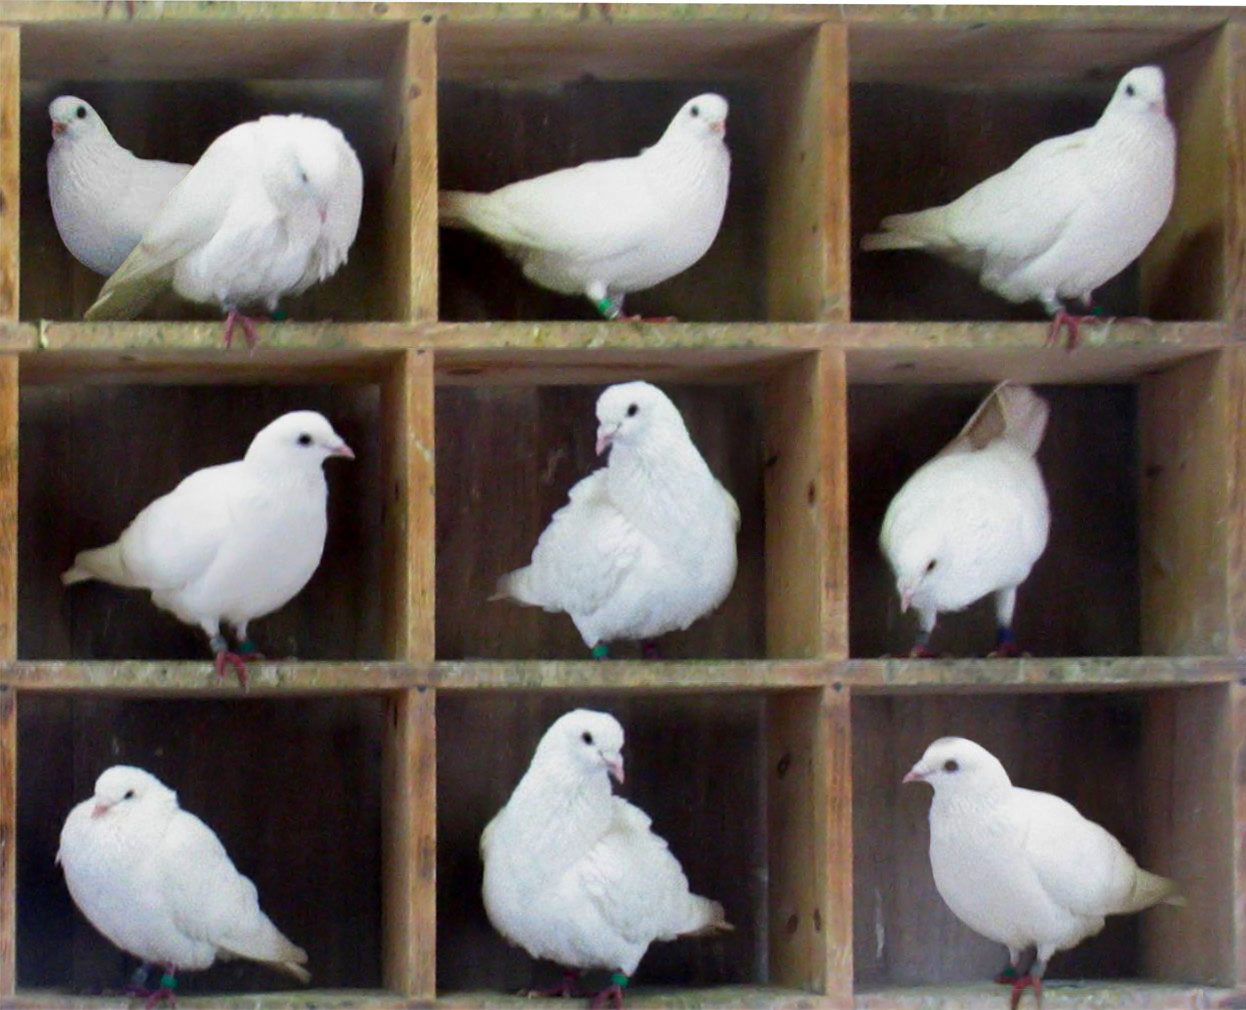
\includegraphics[width = .3\textwidth]{fig/TooManyPigeons.jpg}
\end{center}
\tiny \href{https://commons.wikimedia.org/w/index.php?curid=4658682}{(Wikipedia)}
\end{figure}

\pause
\begin{corollary}[Too few pigeons]
If ${n \choose k}$ is greater than the size of a PRNG's state space, then the PRNG cannot possibly generate all samples of size $k$ from a population of $n$.
\end{corollary}
}


\frame{
\frametitle{Pigeons and Pigeonholes}

Does it matter in practice? 
\pause

\vspace{20pt}

Period of 32-bit linear congruential generators (e.g. RANDU): $2^{32} \approx 4 \times 10^9$ \\
Samples of size $10$ from $50$: ${50 \choose 10} \approx 10^{10}$ \\
\textbf{More than half of samples cannot be generated}
\vspace{20pt}
\pause

Period of Mersenne Twister (standard PRNG in Statistics): $2^{32 \times 624} \approx 2 \times 10^{6010}$ \\
Permutations of $2084$ objects: $2084! \approx 3 \times 10^{6013}$\\
\textbf{Less than $0.01\%$ of permutations can be generated}


}


\frame{
\frametitle{Impossibility bounds}
Let $F$ be the uniform distribution on all samples of size $k$ from a population of $n$.
For some subset of samples $S$,
define $\mathcal{G} = \{ G: G(S) = 0, S \in \mathcal{S}\}$ and $\nu = \lvert S \rvert$.


\begin{lemma}
For any $G \in \mathcal{G}$, $ \lVert F - G \rVert_1 \geq \frac{2\nu}{{n \choose k}}$
\end{lemma}


For any bounded function $\psi: \Omega \to \reals$ and for any $G \in \mathcal{G}$,

$$\left\lvert \int \psi dG - \int \psi dF \right\rvert \leq \lVert F - G \rVert_1 \lVert \psi \rVert_\infty$$


\begin{corollary}
There exists a statistic $\psi$ such that

$$\left\lvert  \ex_F(\psi) - \ex_G(\psi) \right\rvert \geq  \frac{2\nu \lVert \psi \rVert_\infty}{{n \choose k}}$$
\end{corollary}


}

\frame{
\frametitle{Bad seeds}

\bit
\item \textbf{Seed}: an initial value to set the state of a PRNG
\item The choice of seed matters:
\bit
\item Mersenne Twister has problems with seeds with too many zeros \todo{CITE}
\item LCGs may not achieve their full period with certain seeds \todo{CITE}
\eit
\eit

\begin{figure}[htbp]
\begin{center}
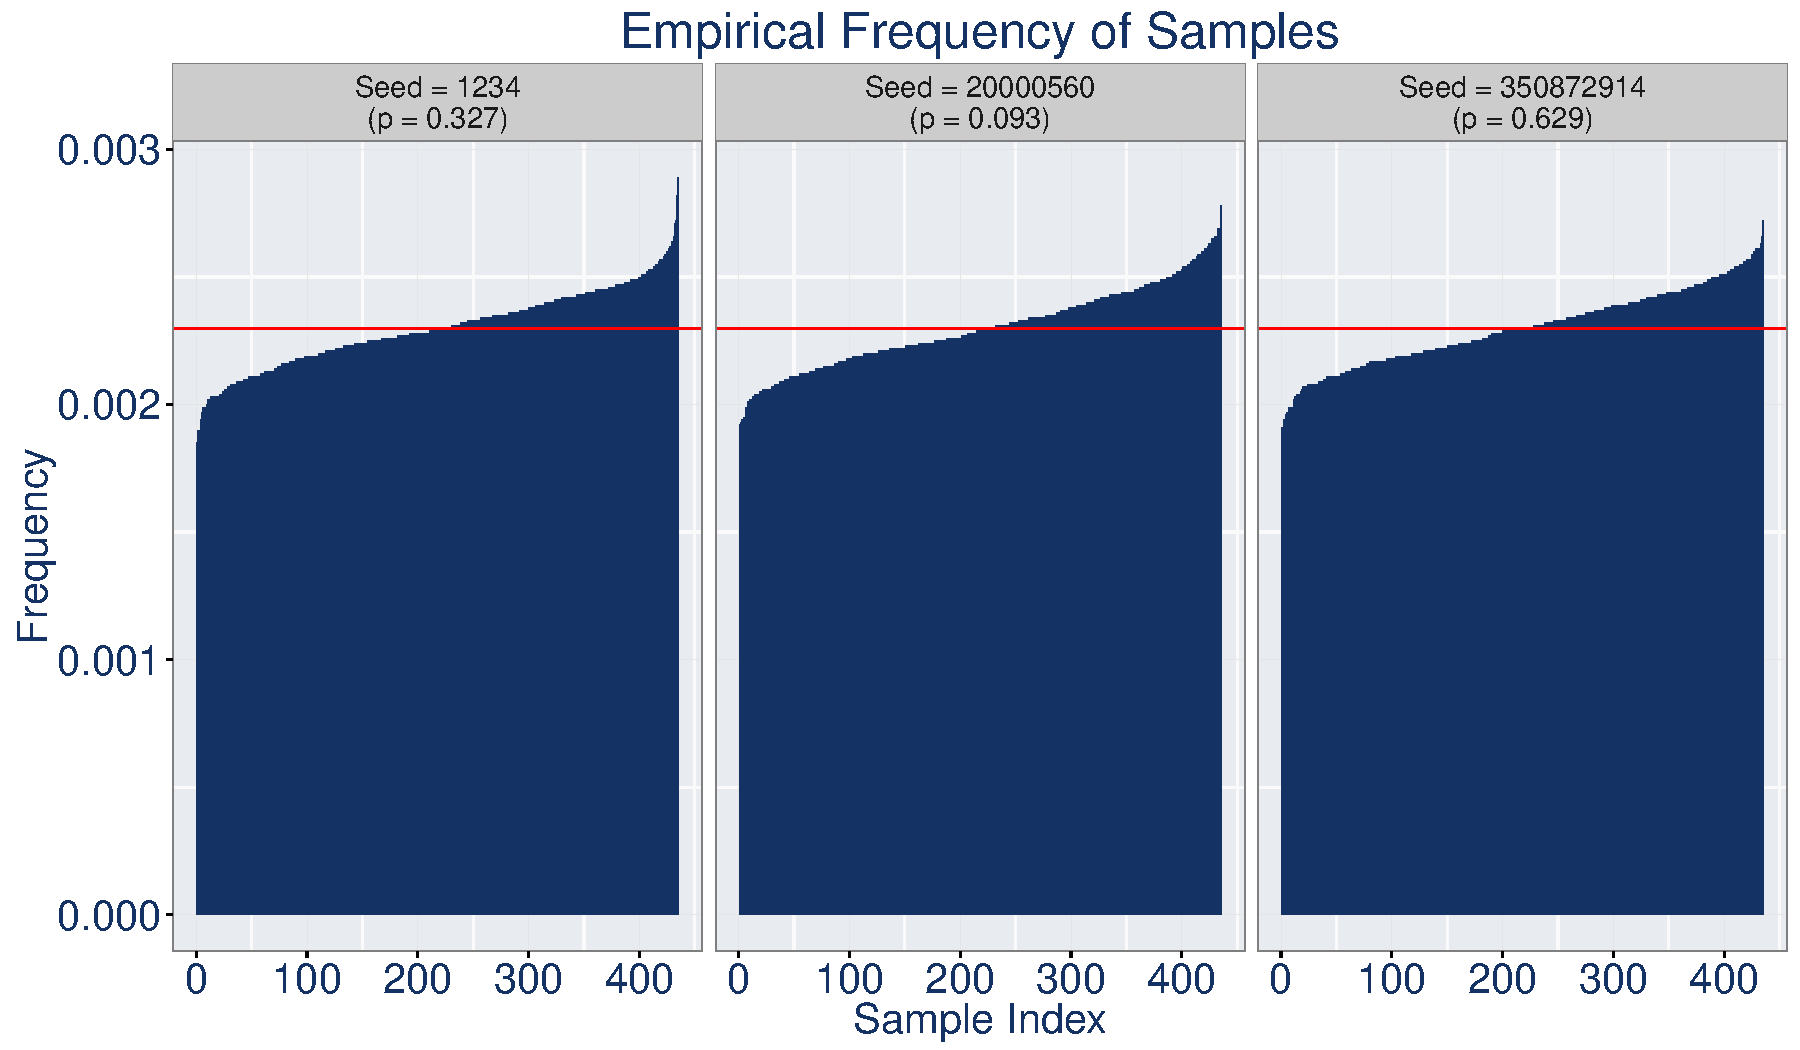
\includegraphics[width = 0.8\textwidth]{fig/bad-seeds.pdf}
\end{center}
\footnotesize{$10^5$ samples of size $2$ from a population of $30$ (Mersenne Twister in R)}
\end{figure}
}

\frame{
\frametitle{Outline}
\bit
\item Better sampling algorithms - resevoir methods
\item Better PRNGs - cryptographic hash functions
\eit
}

\section[Sampling algorithms]{Sampling Algorithms}

\frame{
\frametitle{General idea}

There are two general strategies for sampling algorithms:
\bit
\item ``Shuffle the deck'' and take the top $k$ as the sample
\item Number the population, select $k$ random integers, and sample the corresponding items
\eit
}

\frame{
\frametitle{PIKK}
\begin{algorithm}[H]                      % enter the algorithm environment
\caption{PIKK: Permute indices and keep $k$}          % give the algorithm a caption
\label{PIKK}                           % and a label for \ref{} commands later in the document
\begin{algorithmic}[1]             % enter the algorithmic environment
     \State{Assign IID uniform values on $[0,1]$ to the $n$ elements of the population}
     \State{Sort the population according to these values (break ties randomly)}
     \State{Take the top $k$ to be the sample}
\end{algorithmic}
\end{algorithm}

\bit
%\item Used for sampling in \todo{Stata? can't find the source code or algorithm}
\item Relies on assumption that all permutations are equally likely
\item Inefficient: requires $n$ PRNs and $O(n\log n)$ sorting operation
\item Sort: Stata uses a random sort function to break ties! Not reproducible! \todo{cite http://www.stata-journal.com/sjpdf.html?articlenum=dm0019}
\eit

}




\frame{
\frametitle{Shuffling algorithms}
\bit
\item Knuth shuffle: requires $n-1$ random integers, but no sorting.
\begin{algorithm}[H]                      % enter the algorithm environment
\caption{Fisher-Yates-Knuth-Durstenfeld shuffle}          % give the algorithm a caption
\label{FYKD}                           % and a label for \ref{} commands later in the document
\begin{algorithmic}[1]               % enter the algorithmic environment
\For{$i = 2, \dots, n$}
    \Let{$J$}{random integer uniformly distributed on $1, \dots, i$}
    \Let{$(a[J], a[i])$}{$(a[i], a[J])$}
\EndFor
\State{Take the first $k$ to be the sample}
\end{algorithmic}
\end{algorithm}
\todo{put proof that shuffle works in appendix}
\item Resevoir algorithms: Algorithm R (Waterman, Knuth 1997), Algorithm Z (Vitter 1985) are related to shuffling and don't require knowing the population size a priori
\eit
}


\frame{
\frametitle{Using random integers}
\begin{algorithm}[H]                      % enter the algorithm environment
\caption{Uniform random integers}          % give the algorithm a caption
\label{uri}                           % and a label for \ref{} commands later in the document
\begin{algorithmic}[1]             % enter the algorithmic environment
\Let{$\tilde{n}$}{$n$}
\Let{Population indices}{$\{1, \dots, n\}$}
\For{$i = 1, \dots, k$}
%     \Let{$w$}{a uniform PRN on $[0, 1)$}
%     \Let{$j$}{Element in the $\lfloor\tilde{n}w\rfloor + 1$ space in Population indices}
     \Let{$w$}{A random integer on $\{1, \dots, \tilde{n}\}$}
     \Let{$j$}{The $w$th element in Population indices}
     \Let{Sample indices}{Sample indices $\cup \{j\}$}
     \Let{Population indices}{Put last remaining index in place $j$}
     \Let{$\tilde{n}$}{$\tilde{n}-1$}
\EndFor
\State{Take the items with selected Sample indices}
\end{algorithmic}
\end{algorithm}

\bit
\item Method used by R \texttt{sample}, Python \texttt{random.sample}
\item More efficient: uses only $k$ PRNs and no sorting
\eit
}


\frame{
\frametitle{Generating (non)uniform integers}
\bit
\item Algorithm 2 relies on uniformly distributed integers
\item A common way to get integers in the range $\{1, \dots, m\}$ is $X = \lfloor m U\rfloor + 1$, $U \sim U[0,1)$.
%\bit
%\item $U$ is uniform on $\{0, 2^{-w}, 2\times 2^{-w}, \dots, (2^w - 1)\times2^{-w}\}$
%\item $mU$ is uniform on $\{0, m2^{-w}, 2m\times 2^{-w}, \dots, (2^w - 1)m\times2^{-w}\}$
%\eit
\item Unless $m$ is a multiple of $2^w$, $\lfloor mU \rfloor$ will not truly be uniform!
\eit

\begin{lemma}
For $m < 2^w$, the ratio of the largest to smallest selection probability is, to first order,  $1+ m 2^{-w}$. (See, e.g., Knuth v2 3.4.1.A.)
\end{lemma}
\todo{proper citation, put proof in appendix}
}

\frame{
\frametitle{Generating (non)uniform integers}
A better way to generate integers on $\{1, \dots, m\}$:
\bit
\item Let $w = \lfloor \log_2 m \rfloor + 1$
\item Generate a $w$-bit integer $J$
\item If $J > m$, discard and repeat.
\eit
}

\frame{
\frametitle{Sampling simulations with MT}
\todo{Code up all of the sampling algorithms for Python with numpy.random. Compare how uniform samples are, using the same seed.}

}

\section[PRNGs]{Pseudorandom Number Generators}

\frame{
\frametitle{What makes a PRNG}

\bit
\item Fast and memory efficient
\item Mimics a random sequence (statistically indistinguishable)
\item Unpredictable. this is different from random - if it's deterministic, then it's predictable to some degree
\item Jump-ahead feature so we can efficiently skip random numbers, generate multiple streams for parallel applications
\eit
}



\frame{
\frametitle{Linear Congruential Generators}
LCGs have the form
$$ X_{n+1} = (a X_n + c) \mod m$$

Smart choices of $a$,$c$, and $m$ can make the LCG fast to compute and more or less random

\begin{theorem}[Hull-Dobell Full Period Theorem]
\label{thm:hull_dobell_period}
The period of an LCG is $m$ for all seeds $X_0$ if and only if
\begin{itemize}
\item $m$ and $c$ are relatively prime,
\item $a-1$ is divisible by all prime factors of $m$, and
\item $a-1$ is divisible by 4 if $m$ is divisible by 4.
\end{itemize}
\end{theorem}

}

\frame{
\frametitle{The good, the bad, and the ugly}
\begin{block}{(Knuth, 1997)}
``Random numbers should not be generated with a method chosen at random.''
\end{block}
\pause
\citet{marsaglia_random_1968} proved that $n$-tuples of numbers generated by any LCG will lie on parallel hyperplanes, making them especially non-random.


\begin{figure}[htbp]
\begin{center}
\includegraphics[width = 0.4\textwidth]{fig/randu.png}
\end{center}
     Triples of RANDU lie on 15 planes in 3D space \\ 
     $x_{n+1} = (65539 x_{n}) \mod 2^{31}$ \\
\footnotesize{(Wikipedia)}
\end{figure}
}

\frame{
\frametitle{Linear Congruential Generators}
\bit
\item Fast to compute and requires little memory
\item Some LCGs are more random than others -- depends on choosing good constants
\item Not unpredictable. We only need 2 values to determine the constants.
\item Possible to do jump ahead using mathematical formulas.
\eit
}



\frame{
\frametitle{Mersenne Twister}
explain. state of the art in statistics
}

\frame{
\frametitle{Mersenne Twister}
\bit
\item Fast to compute but has a large state space, not the most memory efficient
\item Random to a good degree
\item Completely predictable after we've seen 623 values
\item No good jump ahead feature
\eit
}



\frame{
\frametitle{A better alternative}

\textbf{One solution:} Find a class of PRNGs with infinite state space
}

\frame{
\frametitle{Hash function PRNGs}

Describe how hash functions work

\begin{center}
\resizebox{10cm}{!}{    
\begin{tikzpicture}[node distance = 1cm, auto, scale = 0.5]
    % Place nodes
    \node [io] (IV) {IV};
    \node [f, right of=IV] (f1) {f};
    \node [f, right of=f1] (f2) {f};
%    \node [f, right of=f2, minimum width = 0cm, height = 0cm] (invisible) {};
    \node [f, right of=f2, node distance=3cm] (fn1) {f};
    \node [f, right of=fn1] (fend) {f};
%    \node [f, right of=invisible, node distance=3cm] (fend) {f};
    \node [f, right of=fend] (g) {g};
    \node [io, right of=g] (hx) {$h(x)$};
    \node [message, above of=f1] (m1) {$x_1$};
    \node [message, above of=f2] (m2) {$x_2$};
    \node [message, above of=fn1] (mn1) {$x_{n-1}$};
    \node [message, above of=fend] (mend) {$x_n$};
    \node [message, above right = of m1, above left = of mend, minimum width = 5cm] (message) {$x$};
    % Draw edges
    \path [line] (IV) -- (f1);
    \path [line] (f1) -- (f2);
    \path [line] (message) -- (m1);
    \path [line] (message) -- (m2);
    \path [line] (message) -- (mn1);
    \path [line] (message) -- (mend);
    \draw [-,dotted] (m2) -- (mn1);
    \path [line] (m1) -- (f1);
    \path [line] (m2) -- (f2);
     \path [line] (mn1) -- (fn1);
    \path [line] (mend) -- (fend);
    \path [line] (fend) -- (g);
    \path [line,dashed] (f2) -- (fn1);
    \path [line] (fn1) -- (fend);
    \path [line] (g) -- (hx);
\end{tikzpicture}
}
\end{center}


Cryptographic hash functions:
\begin{itemize}
\item computationally infeasible to invert
\item difficult to find two inputs that map to the same output
\item small input changes produce large, unpredictable changes to output
\item resulting bits are uniformly distributed
\end{itemize}

}


\frame{
\frametitle{Hash function PRNGs}
Describe procedure with counter
\bit
\item Fast: depends on well-tested hash function code. Number of hashes may slow it down, with the benefit of adding more unpredictability.
\item Memory efficient: Store a seed and a counter -- just like 25 digits
\item Unpredictable: small changes to input produce large unpredictable changes to output. The only way to figure out the sequence is to know the hashing function
\item Jump ahead: just add to the counter.
\eit
}

\section[Results]{Results}

\frame{
\frametitle{Simulations}
\bit
\item Compare PIKK/good sampling algo, MT/CSPRNG/LCG/KISS, different seeds
\item For the unique sample frequencies, report
\bit
\item Range statistic p-value
\item Chi-squared test p-value
\eit
\item Do this for various numbers of samples - 1e6 up to 1e8. This relates to equidistribution
\eit
}


\frame{
\frametitle{Choice of seed}

Preliminary results: the distribution of simple random samples is less uniform if you use a stupid seed

\begin{table}[htdp]
\begin{center}
\begin{tabular}{r|c|c|}
 & $p$-value& $p$-value\\
PRNG &  (seed = 100) &  (seed = 233424280) \\
\hline
RANDU & 0  & 0 \\
Super-Duper LCG & 0.1798 & 1 \\
Mersenne Twister*  & 0.0858 & 0.4741 \\
Mersenne Twister & 0.1996 & 0.6143 \\
SHA-256 PRNG & 0.1710 & 0.8584
\end{tabular}
\end{center}
\label{default}
\end{table}%

\small{* using \texttt{np.random.choice} to sample}

}



\frame{
\frametitle{Open questions}
\begin{itemize}
\itemsep10pt
\item Do ``good'' PRNGs produce all samples with equal probability? All permutations?
\pause
\item Do departures from uniformity introduce bias?
\pause
\item Replace the default PRNGs in Python
\url{https://www.github.com/statlab/cryptorandom}
\pause
\item Results apply more broadly to computer simulations: permutation tests, bootstrapping, MCMC, etc.
\end{itemize}

}


\end{document}
